\documentclass[12pt]{projeto}
\makeatletter
\DeclareRobustCommand{\rm}{\@font@warning{Using old font command \string\rm}\normalfont}
\makeatother
\graphicspath{{figures/}}
% Insira suas informações no arquivo conf.tex
%\usepackage{natbib}
\usepackage[alf]{abntex2cite}
\usepackage{aas_macros} 
\usepackage{array} % Certifique-se de que este pacote está no seu preâmbulo.

%\usepackage{fontspec}

%%%%%%%%%% Arquivo de configuração do projeto
%% Insira seus dados e modifique o modelo com suas preferências
%% Comente/descomente linhas para modificar o modelo
%% Aviso! O modelo não segue uma norma específica

%%%%%%%%%%%%%% Informações dos projeto
\tipo{Relatório Final IC - Bolsa PIBIC}
\titulo{Investigando o Efeito Sintético em Modelos Espectrais de Populações Estelares}
\aluno{André Almeida Trovello}
\emailaluno{andretrovello@usp.br}
\orientador{Paula R. T. Coelho}
\emailorientador{pcoelho@usp.br}
\palavraschave{Projeto, Mestrado, Galáxias disco, Populações Estelares}
\data{\today}

%%%%%%%%%%%%%% Pacotes extras
\usepackage{lipsum} % Gera texto dummy
%\usepackage{fullpage} % Uniformiza as margens (1,5 cm) 
\usepackage{xcolor}
\usepackage{geometry}
\geometry{margin=1in}

%%%%%%%%%%%%%% Bibliografia
%% Para referências estilo ABNT tire o comentário de uma das linhas 
%% Manual do pacote de referências: https://www.abntex.net.br/

%\usepackage[num]{abntex2cite}	% Referências numéricas padrão ABNT
%\usepackage[alf]{abntex2cite}  % Referências alfabéticas padrão ABNT

\AtEndDocument{
    \bibliografia{bibtex.bib} % Arquivo com o bibtex
    \estilobibliografico{apalike} % Estilo das referências se não usar ABNT
%% Mais estilos: https://www.overleaf.com/learn/latex/bibtex_bibliography_styles
}

%% Para adicionar backrefs tire o comentário da linha abaixo,
%% backrefs listam as paginas em que uma referência foi citada
%\usepackage[brazilian,hyperpageref]{backref} % Adiciona backrefs

%%%%%%%%%%%%%% Confs
\AtBeginDocument{
    \maketitle % Gera cabeçalho
    \pagestyle{plain} % Efetivamente, insere a numeração
}

%%%%%%%%%%%%%%%% Comandos úteis para matemática
\newcommand{\Z}{\mathbb{Z}}
\newcommand{\Q}{\mathbb{Q}}
\newcommand{\R}{\mathbb{R}}
\newcommand{\trans}{^\intercal}
\newcommand{\pc}[1]{\texttt{\textcolor{magenta}{[#1]}}}

\DeclareMathOperator{\posto}{posto}
\DeclareMathOperator{\capacidade}{cap}
\DeclareMathOperator{\valor}{val}
\DeclareMathOperator{\mdc}{mdc}
\DeclareMathOperator{\adj}{adj}
\DeclareMathOperator{\conv}{conv}
\DeclareMathOperator{\cone}{cone}

\DeclarePairedDelimiter\ceil{\lceil}{\rceil}
\DeclarePairedDelimiter\floor{\lfloor}{\rfloor}

\newtheorem{teorema}{Teorema}
\newtheorem{definicao}{Definição}
\newtheorem{lema}{Lema}
\newtheorem{proposicao}{Proposição}
\newtheorem{corolario}{Corolário}
\newtheorem{fato}{Fato}
\theoremstyle{definition} % Arquivo de configuração

\begin{document}

\begin{abstract}
Modelos de síntese de população estelar nos possibilitam estudar e obter as propriedades de galáxias ou aglomerados a partir de seus espectros integrados. Como todo modelo, estes apresentam imprecisões, podendo elas estarem relacionadas à evolução estelar, função de massa inicial ou ao tipo de espectro estelar utilizado. Os modelos podem ser construídos a partir de bibliotecas estelares empíricas ou teóricas, dos quais as limitações estão relacionadas à cobertura do diagrama HR, no primeiro caso, e ao limite de conhecimento físico que possuímos sobre as atmosferas estelares, no segundo. A literatura se refere ao ``efeito sintético'' como sendo as alterações nos modelos de população estelar que ocorrem quando uma biblioteca estelar empírica é trocada por uma teórica. Este projeto possui como objetivo verificar as diferenças entre modelos de população estelar, comparando os modelos baseados na biblioteca estelar empírica MILES com os modelos baseados na biblioteca teórica SynCoMiL. Esperamos estudar os efeitos sintéticos, identificando assim as regiões do espectro que mais divergiram e necessitam ser modeladas com maior atenção. Neste primeiro semestre de iniciação científica foram desenvolvidas as seguintes atividades: estudo bibliográfico, manuseamento e limpeza de dados, e reprodução de resultados prévios da literatura. A primeira englobou todo o estudo astronômico sobre modelos de população estelar e técnico (Python e R). A segunda envolveu o aprimoramento dos meus conhecimentos em tratamento de dados. Já a última ateve-se a reproduzir resultados disponíveis na literatura, como forma de verificar se os algoritmos utilizados em meus códigos estavam corretos e poderiam ser utilizados para avaliar novos modelos. Os resultados obtidos se mostraram parcialmente compatíveis com os apresentados no artigo tomado como base para este projeto. No cálculo de diferenças de índices normalizadas, porém, há uma discrepância cuja origem não foi identificada, havendo a suspeita de que esta ocorreu devido ao diferente funcionamento das bibliotecas do Python e do R. 
\end{abstract}


\section{Introdução}

A determinação de distâncias é uma questão relevante na astronomia contemporânea. Em especial, a determinação de distâncias de aglomerados estelares se mostra primordial para refinar modelos de formação e evolução estelar, visto que o cálculo dessa grandeza possibilita a conversão de valores aparentes de magnitudes em absolutos, viabilizando a obtenção acurada de parâmetros como idade e massa das estrelas que compõem o aglomerado.

Tradicionalmente, a distância destes aglomerados é calculada pela inversão das paralaxes observadas em seus membros, porém, este método se mostra altamente sujeito a erros aleatórios quando são estudados aglomerados mais distantes, já que nestas ocasiões o erro da paralaxe pode apresentar mesma ordem de grandeza que a própria paralaxe em si.

No contexto deste problema, a missão espacial Gaia \cite{gaia_collaboration_gaia_2016} contribuiu significativamente, fornecendo paralaxes de alta precisão de aglomerados e estrelas. Como toda medida experimental, os dados da Gaia possuem um erro associado, sendo este uma combinação de três fatores principais: erros aleatórios (a incerteza estatística individual de cada fonte), erros sistemáticos (oriundos de fatores como posição, cor e magnitude da estrela, que afetam estrelas próximas no céu de maneira semelhante) e o zero point (um offset de medição sistemático associado ao próprio instrumento Gaia).

Em decorrência da propagação não linear das incertezas da paralaxe, técnicas como a Inferência Bayesiana se mostram como boas alternativas para contornar essa questão, possibilitando calcular a distribuição de probabilidade posterior das distâncias de aglomerados, incorporando a verossimilhança dos dados observados e o conhecimento prévio através dos priors.

Baseado nessa técnica, o código Kalkayotl \cite{olivares_kalkayotl_2020} foi desenvolvido utilizando um framework bayesiano hierárquico para inferir simultaneamente os parâmetros da população e as distâncias individuais das estrelas. Sua abordagem tem a vantagem de tratar as correlações espaciais das paralaxes, provendo estimativas confiáveis de distância e incertezas não subestimadas. 

Este projeto teve como objetivo determinar a distância de um aglomerado aberto por meio do código Kalkayotl 1.0, comparando seus resultados com os publicados na literatura, de forma a visualizar a eficácia do método bayesiano quando confrontado com outras estimativas, e compreender quais priors se adequam melhor ao aglomerado em questão. 

\subsection{Aquisição de Dados e Seleção do Aglomerado}

Os dados de aglomerados foram obtidos a partir do catálogo de Emily L. Hunt \cite{hunt_improving_2024}, que através das medições do Gaia DR3 \cite{vallenari_gaia_2023}, fez um estudo de 6956 aglomerados classificados por trabalhos prévios e verificou a ligação gravitacional de suas estrelas membros, concluindo que apenas 5647 (79\%) deles podem ser considerados abertos, fornecendo também estimativas de distâncias para estes corpos celestes. 

Definido o método e o catálogo analisado, fez-se necessária a determinação de um aglomerado para estudo. Para evitar dificuldades no cálculo da distância, utilizou-se como critério de seleção a proximidade do aglomerado (\(<500\)pc) e a quantidade de estrelas membros (\(>200\)). Dessa forma, foi escolhido o aglomerado NGC 1662 (Figura \ref{fig:NGC1662}), composto por \(384\) estrelas e a (\(404,59 \pm 0,28\)) parsecs de distância, segundo o catálogo de Hunt.
\begin{figure}[ht]
\centering
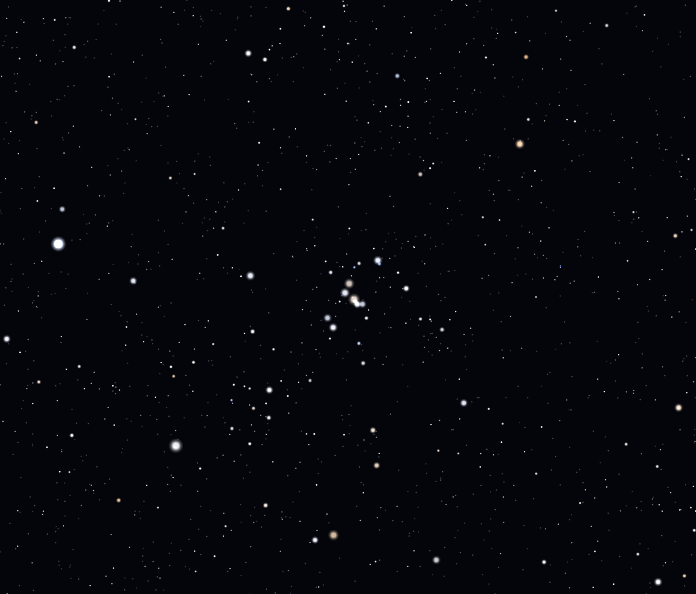
\includegraphics[width= 0.8\textwidth]{NGC_1662.png}
\caption{\label{fig:NGC1662} Aglomerado NGC 1662.}
\end{figure}

\subsection{Revisão da Literatura e Metodologias de Distância}

A estimativa de distância do aglomerado NGC 1662 foi contextualizada e comparada com quatro catálogos notáveis (Tabela \ref{tab:comparativo_distancias_incerteza}) , que ilustram a evolução das metodologias na astrometria galáctica: um catálogo pré-Gaia \cite{dias_new_2002}, dois trabalhos do Gaia DR2 com diferentes abordagens \cite{cantat-gaudin_painting_2020, dias_updated_2021} e um catálogo moderno do Gaia DR3 \cite{hunt_improving_2024}.

Na primeira abordagem, o catálogo DIAS et al., (\citeyear{dias_new_2002})  realizou uma compilação de valores de distância da literatura calculados pelo ajuste da sequência principal fotométrica no Diagrama Cor-Magnitude (CDM) e, no caso de aglomerados próximos, pela inversão da média das paralaxes calculadas pelo satélite Hipparcos \cite{esa_hipparcos_1997}. Para NGC 1662, foi estimada uma distância de \(437\) parsecs, utilizando o método fotométrico. Dado que utilizou de dados de baixa precisão de missões antigas, este método não apresentou incerteza em sua medida.

Com a precisão do Gaia DR2 \cite{gaia_collaboration_gaia_2018}, surgiram métodos mais robustos de determinação de parâmetros, embora com diferentes estratégias para o tratamento de erros. CANTAT-GAUDIN et al., (\citeyear{cantat-gaudin_painting_2020}) utiliza de um modelo de Inferência Bayesiana Hierárquica para inferir a distribuição de probabilidade das paralaxes dos membros de aglomerados, de onde a distância final é obtida por meio da mediana da distribuição de probabilidade \textit{a posteriori}. Embora tenha sido validado, as incertezas finais deste método não foram fornecidas no catálogo, limitando a avaliação de confiabilidade do valor de \(428\) parsecs obtido para NGC 1662.

Por sua vez, \cite{dias_updated_2021} realizou o cálculo de distâncias por meio do ajuste de isócronas (\textit{isochrone fitting}) ao CDM, empregando o algoritmo de entropia cruzada para determinar parâmetros como a distância, idade, extinção e metalicidade. O método incluiu a aplicação de priors e utilizou reamostragem Monte-Carlo (\textit{bootstrapping}) para a determinação das incertezas, obtendo assim um valor de (\(410 \pm 3\)) parsecs para NGC 1662.

Com o advento do Gaia DR3, o aumento na precisão astrométrica permitiu a HUNT; REFFERT,.(\citeyear{hunt_improving_2024}) calcular distâncias novamente por ajuste de isócronas ao CDM. Entretanto, o método foi aprimorado com um estudo estatístico que visa o máximo rigor. A identificação de membros do algomerado é feita pelo algoritmo HDBSCAN (Hierarchical Density-Based Spatial Clustering of Applications with Noise - CAMPELLO; MOULAVI; SAN-
DER \citeyear{campello_density-based_2013}), e a distância final é o resultado de um processo de inferência probabilística de parâmetros. Por ser um método estatístico avançado e de natureza bayesiana em seus resultados, o catálogo fornece a distância como a mediana (50º percentil) da distribuição de probabilidade, acompanhada dos limites do Intervalo Crível (16º e 84º percentis), resultando em nosso último valor de comparação para NGC 1662 de (\(404,60 \pm  0,28\)) parsecs. 


\begin{table}[ht]
    \centering
    \caption{Comparativo das estimativas de distância para NGC 1662 e suas incertezas (quando calculadas).}
    \label{tab:comparativo_distancias_incerteza}
    % Redefinindo o ambiente tabular para usar alinhamento vertical 'm'
    % Adicionamos '\renewcommand{\arraystretch}{1.5}' para um espaço extra uniforme
    \renewcommand{\arraystretch}{1.3} % Aumenta o espaçamento padrão
    \begin{tabular}{|>{\centering}m{5cm}|>{\centering\arraybackslash}m{4cm}|}
        \hline
        \textbf{Autor (Ano)} & \textbf{Distância ($d$) [pc]} \\
        \hline
        Hunt et al. (2024) & $404,60^{+0,28}_{-\text{0,28}}$ \\
        \hline
        Dias et al. (2021) &  $410^{+3}_{-\text{3}}$ \\
        \hline
        Cantat-Gaudin et al. (2020) & $428$ \\
        \hline
        Dias et al. (2002) & $437$ \\
        \hline
    \end{tabular}
    \renewcommand{\arraystretch}{1.0} % Retorna ao padrão
\end{table}

\subsection{Seleção da Amostra}

O estudo de distância do aglomerado NGC 1662 no Kalkayotl foi feito com duas amostras distintas. A primeira, denominada amostra completa (\(A_{full}\)), incluiu todas as 384 estrelas fornecidas inicialmente pelo catálogo de Hunt. 

Entretanto, para descartar a presença de \textit{outliers} que pudessem enviesar o resultado, realizou-se uma segunda seleção (\(A_{cut}\)), onde foram removidas estrelas que estivessem a uma distância de \(2\sigma\) da mediana do conjunto de dados (Figura \ref{fig:selecao_amostral}). Esta filtragem resultou em uma amostra final de 360 estrelas, que foi então utilizada para o cálculo da distância do aglomerado no Kalkayotl.

\begin{figure}[ht]
\centering
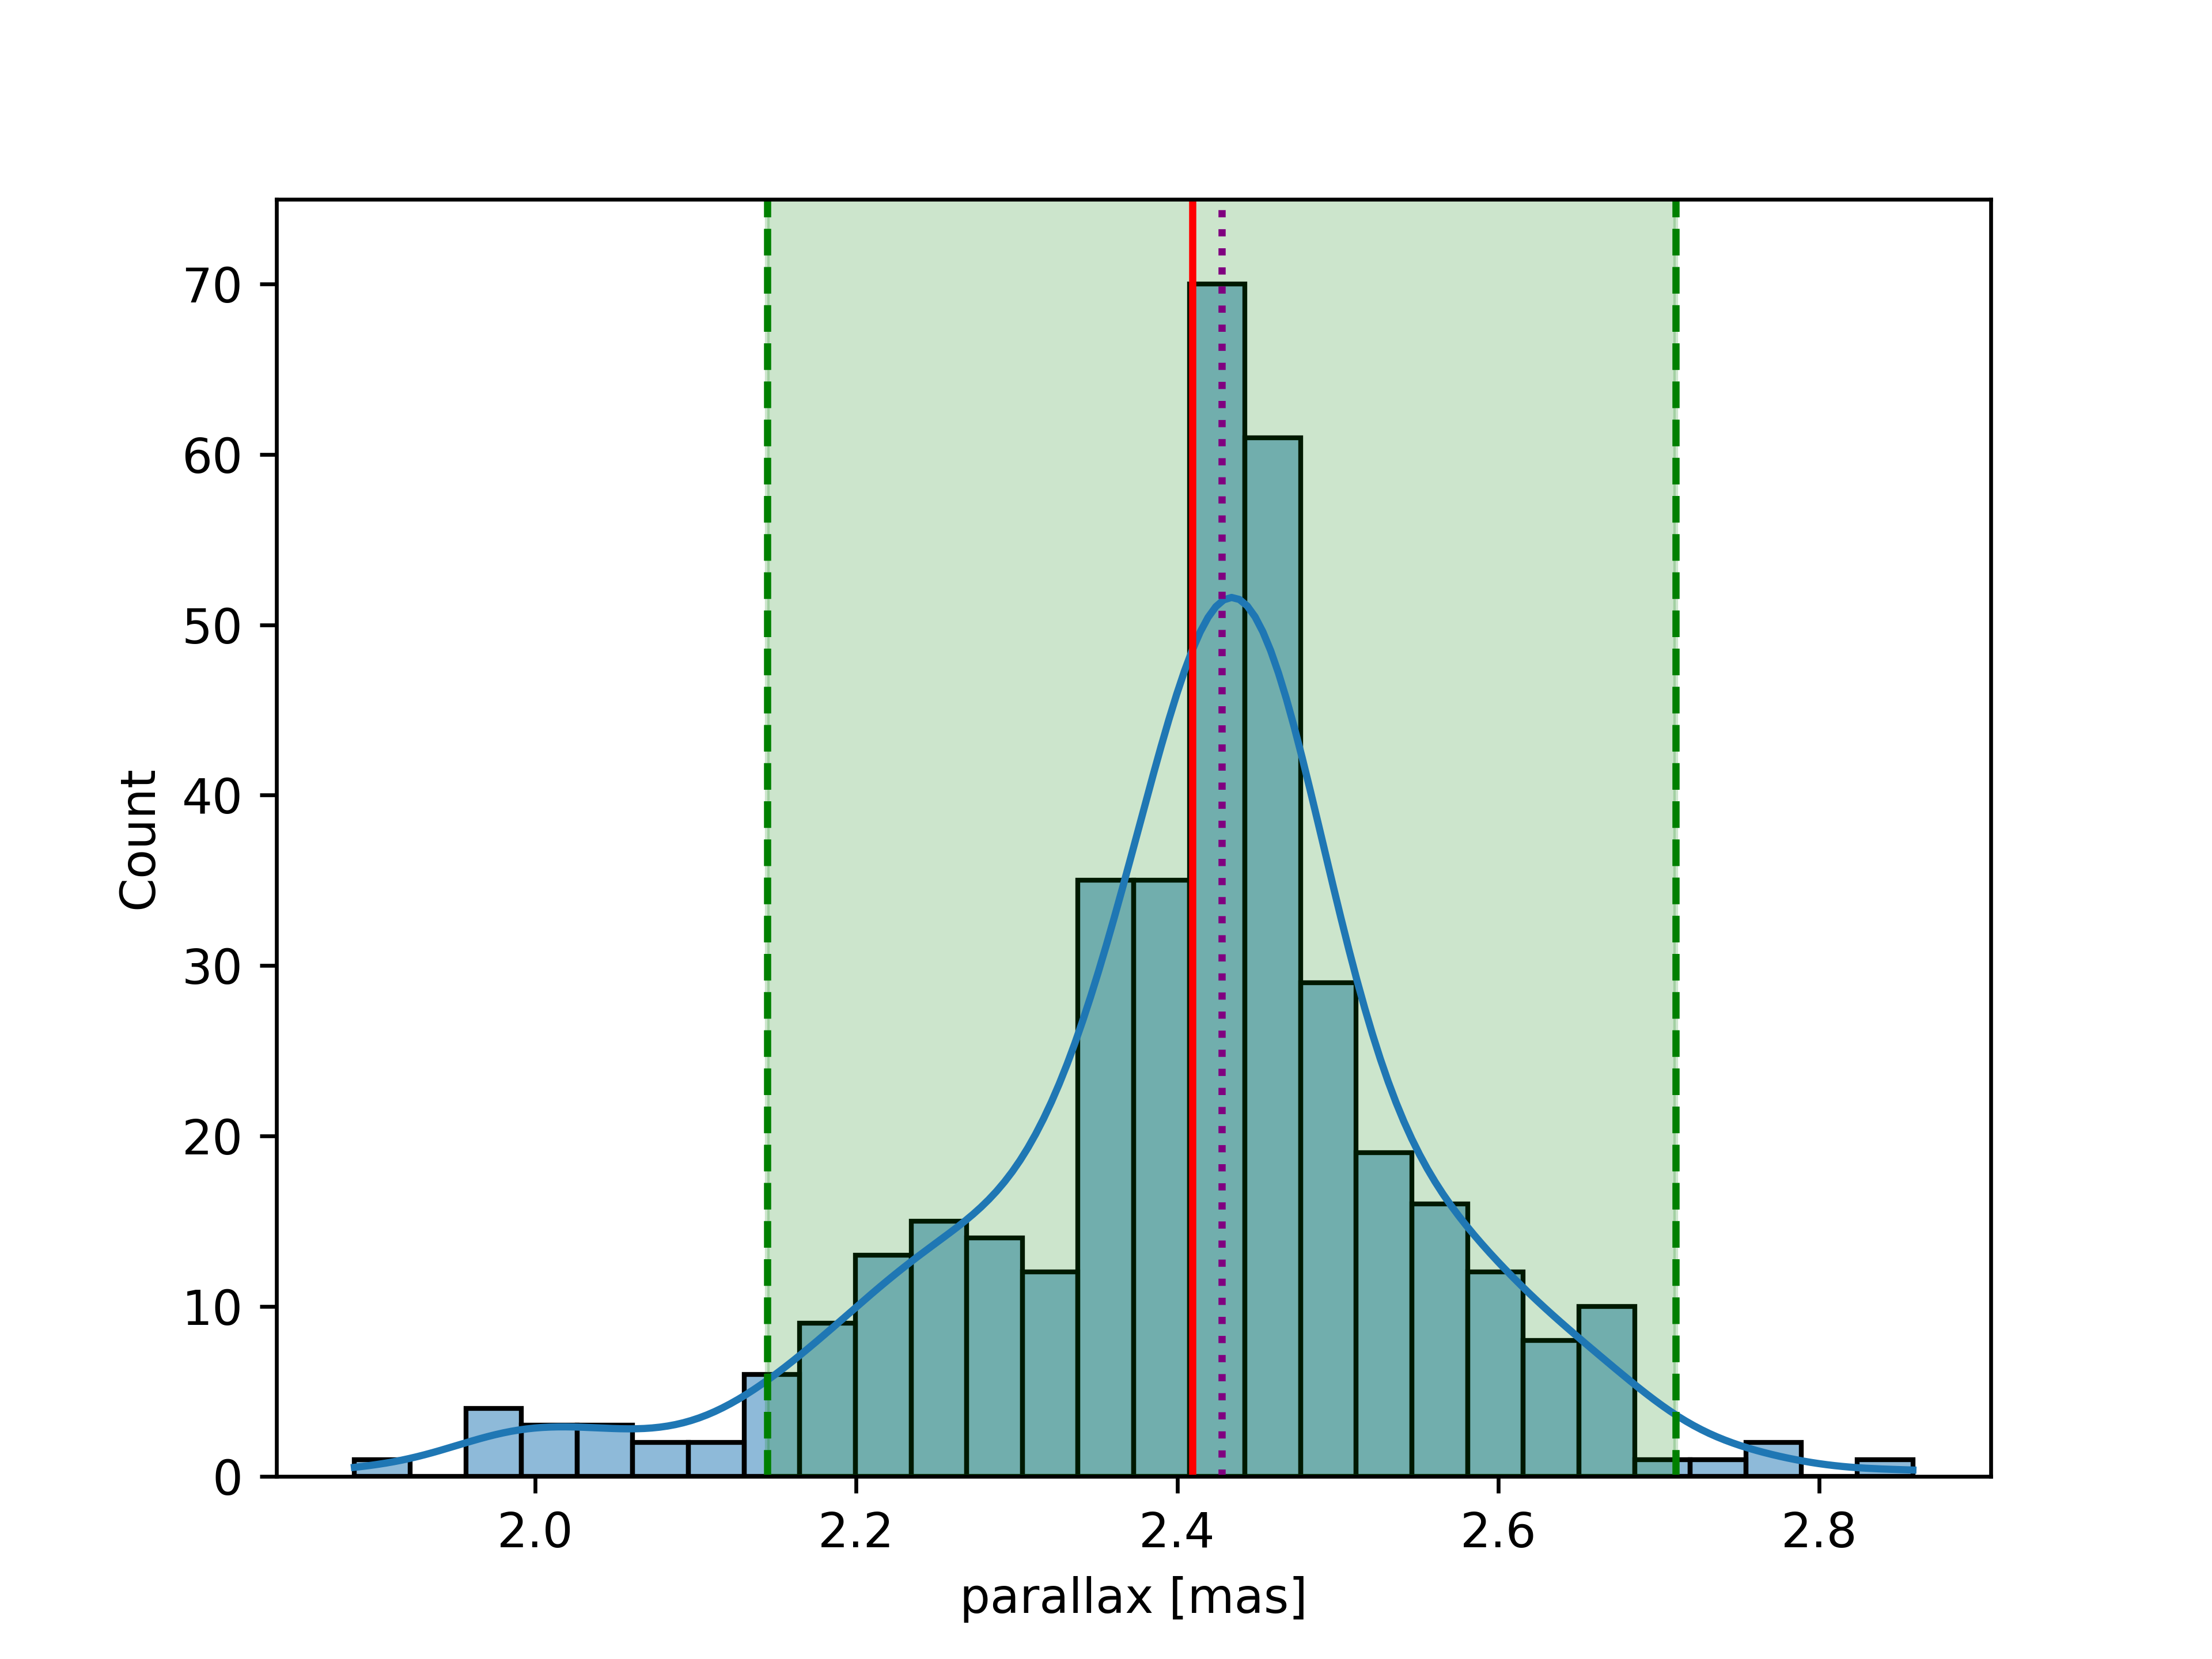
\includegraphics[width= 0.8\textwidth]{NGC1662_parallax.png}
\caption{\label{fig:selecao_amostral} Distribuição dos valores de paralaxe para o aglomerado NGC 1662, bem como a seleção amostral (área verde clara) para \(2\sigma\) (95\%) da mediana (linha pontilhada roxa). Foi escolhida a mediana em detrimento da média (linha vermelha) devido à primeira se aproximar melhor da Estimativa de Densidade de Kernel (KDE, curva verde escura).}
\end{figure}

\subsection{Priors}

\section{Desenvolvimentos}
Neste primeiro semestre de projeto, as atividades se dividiram em três etapas: estudo bibliográfico, manuseamento e limpeza dos dados e reprodução de resultados prévios da literatura.

\subsection{Estudo Bibliográfico}
Esta primeira etapa teve como finalidade adquirir os conhecimentos necessários para o entendimento, tanto do aspecto astronômico do projeto, quanto do técnico. Dessa forma, inicialmente foi feita a leitura e compreensão de artigos sobre modelos de população estelar \cite{BC03}, bibliotecas teóricas e empíricas, bem como as diferenças entre o efeito sintético e de cobertura \cite{Paula2014} e \cite{Paula2020}. Além disso, sabendo que o último passo do projeto visava utilizar o código Starlight \cite{starlight}, foi feito também um estudo desta ferramenta,
capaz de, a partir de modelos de síntese de população estelar, destrinchar o percentual de SSPs que compõem uma galáxia observada, além de estimar sua idade, metalicidade e extinção visual.

Compreendida a astronomia, foi então estudada a questão técnica do projeto, centrada basicamente em programação. Dentre todas as possíveis linguagens para a execução das tarefas necessárias, foram escolhidas Python e R pela sua grande versatilidade em análise de dados, sendo a primeira utilizada de fato, e a segunda servindo como base para comparação visto que a orientadora deste projeto, Prof. Paula R. T. Coelho, possui grande experiência com R, fornecendo assim códigos que pudessem ser estudados para compreender a lógica por trás deles.

Assim, no Python, foram estudadas principalmente as bibliotecas \textit{Numpy}, capaz de realizar operações complexas em arrays, \textit{Pandas}, que possibilita o manuseamento de dados, e \textit{Matplotlib}, que permite a visualização deles. Já no R, foi dada muita ênfase à biblioteca \textit{Tidyverse}, robusto pacote de análise de dados capaz de realizar todas as tarefas já citadas anteriormente.

\subsection{Manuseamento e Limpeza de Dados}

Encerrada a primeira etapa teórica, foi então o momento de iniciar de fato a prática, ou seja, aplicar todos os conhecimentos adquiridos para manusear e limpar os dados dos modelos de população estelar.

Foram acessados três modelos, apresentados em \cite{Paula2020}. O primeiro, nomeado cbc, comporta a biblioteca teórica Coelho 14 (C14), que possui uma extensa cobertura do diagrama Hertzprung-Russel (HRD). Neste caso, os arquivos dividem-se em dois formatos: FITS e gz. 

Flexible Image Transport System (FITS) é um formato de arquivo muito utilizado em astronomia, capaz de carregar consigo diferentes tipos de informação em formatos variados, sendo eles unidades de dados (HDUs) formados por vetores 1D, 2D ou 3D multi dimensionais, além de ASCII headers capazes de transportar informações adicionais ou introdutórias, como coordenadas. Com essa alta flexibilidade e capacidade de armazenamento, diferentemente de imagens convencionais, FITS permite guardar quantidades considerávis de dados que facilitam visualização e análise. Para a leitura deste formato de arquivo, foi utilizada a biblioteca astropy, construída com foco em resolver questões astronômicas em Python.

Já gz é um arquivo compactado utilizando o software GNU zip (gzip), muito utilizado no Linux e Windows.

O segundo modelo (SPS-M) comporta a MILES, uma biblioteca empírica que possui o fluxo calibrado de aproximadamente
1000 estrelas, cobrindo a faixa de 3540-7410Å do espectro eletromagnético. Já o último modelo (SPS-S) utiliza da biblioteca teórica SynCoMiL, que apresenta todas as suas estrelas geradas por modelagem física, porém, foi limitada a apresentar exatamente a mesma cobertura em termos de comprimento de onda e HRD que a MILES. Tanto na SPS-M quanto na SPS-S, os arquivos foram apresentados nos formatos FITS e txt.


Abertos os arquivos no Python, iniciou-se o procedimento de limpeza dos dados. Foram então removidos os índices que apresentavam dados idênticos em todas as linhas e filtrada a base de dados para que fossem apenas utilizados os pontos onde \(7 \leq log age \leq 10\), sendo log age o logaritmo da idade das populações estelares do modelo. Feito isso, foi concluído o tratamento dos dados, permitindo assim a etapa de visualização e análise destes. 


\subsection{Reprodução de Resultados Prévios da Literatura}
A última tarefa deste primeiro semestre foi a reprodução de resultados prévios apresentados na literatura. Dado que o processo de análise e comparação das bibliotecas é o mesmo em todos os casos, para poder avaliar a qualidade de novos modelos de população estelar foi necessário primeiramente verificar se os algoritmos utilizados no Python reproduziam os mesmos resultados obtidos na literatura. Se isso fosse confirmado, era possível inferir então que os códigos utilizados estavam corretos, podendo assim serem aplicados em modelos mais recentes.

Dessa forma, iniciou-se então um procedimento de reproduzir as figuras do trabalho publicado por minha orientadora em \cite{Paula2020}, dando ênfase naquelas que evidenciavam o efeito sintético, objeto de estudo deste projeto. Desta maneira, a primeira tentativa de reprodução foi a da figura 8 do artigo, apresentada na figura  deste projeto. Estes plots demonstram uma comparação direta entre os índices espectrais dos modelos SSP calculados com as bibliotecas MILES  e SynCoMiL, sendo possível observar por meio de uma linha 1-1, ou seja, uma reta \(f(x) = x\), se estes resultados são equivalentes ou não.



Os resultados reproduzidos por mim estão apresentados na figura .
Analisando as figuras obtidas, nota-se que a reprodução dos resultados do artigo foi atingida com sucesso, visto que, em todos os casos, os plots foram equivalentes. Além disso, é perceptível que na maioria dos índices os pontos se mantiveram sobre a linha 1-1, indicando igualdade entre as duas bibliotecas. 

Entretanto, alguns índices apresentaram divergências consideráveis, sendo eles Ca4227, Fe4668, Mg1, Mg2, Fe5406, Fe5709 e B4000Vn. Nestes casos, houve uma disparidade entre os valores da MILES (SPS-M) e SynCoMiL (SPS-S), onde os pontos acabaram distoando da linha 1-1. Além disso, houveram casos como H83889, H93885 e H103798 onde, apesar de haver equilíbrio sobre a linha 1-1, houve uma dispersão maior dos pontos em torno dela, sendo interessante estudá-los também. 


Após a confecção da figura , houveram algumas dificuldades na tentativa de criar as próximas figuras. Primeiramente, tentou-se reproduzir a parte correspondente ao efeito sintético da figura 11 do artigo, visto que esta utilizava do mesmo grupo de dados que as figuras anteriormente mostradas. Neste caso, foi feito um boxplot das diferenças entre os valores dos índices espectrais das bibliotecas MILES e SynCoMiL (\(\Delta idx\)):

\[\Delta idx = I_{SPS-M} - I_{SPS-S}\]

em que I é qualquer índice espectral. Feita esta subtração, foi então aplicada uma normalização da forma

\[z = \frac{x-\mu}{\sigma}\]

onde z é definido pela subtração do valor inicial de \(\Delta idx\) (x) pela média do conjunto (\(\mu\)), sendo este resultado dividido pelo desvio padrão (\(\sigma\)). Os resultados obtidos no artigo estão contidos na figura .

O boxplot gerado pelo Python para reproduzir o artigo está contido na figura .
É perceptível, quando comparados o plot do artigo com aquele feito por mim que houve grande diferença entre eles. Nota-se que, enquanto a figura  apresentou uma crescente nos resultados, indo de valores médios de -2,5 a aproximadamente 0, a média da figura  se manteve centrada neste segundo valor, não havendo muita variação em torno desta região. Além disso, os tamanhos das caixas em cada índice não correspondem aos obtidos por minha orientadora e seus colaboradores, demonstrando que não houve compatibilidade entre eles.

Antes de discutir o por quê esta divergência pode ter ocorrido, vamos fornecer mais um exemplo.

Outra plot que tentou-se refazer, foi o gráfico de densidade presente na figura 7 do artigo (reproduzido nesse texto na figura ). Neste caso, foram utlizados os valores de \(\Delta idx\) calculados anteriormente e plotadas suas densidades.

Novamente com o objetivo de estudar e enfatizar o efeito sintético, foram plotados os gráficos apenas referentes a ele, apresentados na figura .
Avaliando as figuras e , percebe-se mais uma vez que não houve correspondência entre os resultados. Quando analisado o eixo x, é notável que, em alguns casos, a largura da distribuição não apresentou o tamanho esperado, como para os índices TiO1 e TiO2, onde, apesar das distribuições apresentarem a mesma forma, no artigo foi obtida uma ordem de grandeza de \(10^{-2}\), enquanto nos meus resultados, esta foi de \(10^1\). Outro fator interessante é o fato de, em alguns casos, o formato da distribuição divergir, como no caso do índice Fe5015, em que os picos do artigo e deste projeto aparentam estar invertidos. 

Muitas foram as tentativas para avaliar e identifcar o motivo dos resultados estarem se diferenciando tanto. A princípio, foi levantada a hipótese de eu estar manuseando de maneira errada os arquivos FITS, sendo então estes substituídos pelo formato txt. Entretanto, após a troca, a diferença persistiu.

Após isso, o foco foi mudado não para o formato do arquivo e como utilizá-lo, mas sim para as operações matemáticas que estavam envolvidas, já que, em todos os casos problemáticos, houve algo em comum: a subtração dos valores dos índices (\(\Delta idx\)). Assim, foi inicialmente debatido que pode ter ocorrido uma falta de correspondência nos valores subtraídos, ou seja, \(\Delta idx\) estava sendo calculado realizando a diferença de valores espectrais com idades diferentes. Dessa forma, foi então realizada uma correlação cruzada entre as tabelas MILES e SynCoMiL considerando os fatores log age e metalicidade (Z) como determinantes. Apesar de resultar em um formato mais parecido com o esperado nas densidades (figura), ainda assim algumas diferenças persistiram.

Foi cogitado, por fim, que a utilização de linguagens de programação distintas pode ter causado erro nos resultados finais. Originalmente, os plots e a análise do artigo foram todos feitos em R, enquanto neste projeto foi usado o Python. Obviamente, isto não deveria afetar os plots, já que ambas são linguagens muito robustas e muito competentes no tratamento de dados. Entretanto, visto que cada uma delas possui bibliotecas diferentes, estas possuem nuances em suas funções embutidas que podem ter feito com que as operações matemáticas fossem feitas de formas distintas, resultando assim nestes resultados incompatíveis.

Infelizmente não foi possível encontrar o motivo principal destes problemas, visto que, como me graduei, não darei seguimento nas atividades da IC, partindo agora para a pós graduação. Entretanto, como continuarei trabalhando com astronomia extragalática, Python e R, utilizarei os conhecimentos e hipóteses levantados ao longo deste projeto em minhas futuras pesquisas. 

\section{Desempenho Acadêmico}
No segundo semestre de 2024, referente à primeira metade da minha iniciação científica, estive matriculado nas disciplinas de 'Introdução à Cosmologia Física' e 'Introdução ao Caos' nas quais fui aprovado com as médias finais 7,5 e 9,1, respectivamente. Além disso, concluí todos os créditos requeridos pelo meu curso, me graduando assim no Bacharelado em Física pelo Instituto de Física da Universidade de São Paulo (IFUSP). Fui aceito no programa de Mestrado em Astronomia do IAG, onde continuarei minhas atividades acadêmicas.

\section{Conclusões e Perspectivas}

Ao longo deste projeto de IC, foi possível conhecer mais sobre a definição e os usos de modelos de síntese de população estelar, bem como sobre programação, tratamento de dados e análise estatística.

Ao longo do semestre, foram desenvolvidas as atividades de estudo bibliográfico, onde pude compreender mais sobre o funcionamento dos modelos e sobre o modo de operação das linguagens Python e R; manuseamento e limpeza de dados, em que me foi permitido trabalhar diretamente com os modelos de população estelar, compreendendo mais sobre como filtrar e administrar conjunto de dados; e reprodução de resultados prévios da literatura, na qual foram refeitos os gráficos publicados no artigo base deste projeto.

Estes resultados obtidos foram parcialmente compatíveis com o esperado. Para comparações diretas entre os índices espectrais de modelos construídos com as bibliotecas MILES e SynCoMiL, nossos resultados reproduzem os da literatura, revelando semelhança grande entre as bibliotecas. Além disso, foram evidenciados também alguns índices espectrais divergentes que merecem ser reelaborados, como Ca4227, Fe4668, Mg1, Mg2, Fe5406, Fe5709 e B4000Vn.

Já quando foi feito o cálculo de diferenças de índices normalizados, não houve reciprocidade entre os resultados obtidos aqui e os da literatura, de forma que foram cogitados diversos fatores que pudessem ter acarretado essa questão, sendo o mais provável algo relacionado às diferenças de funcionamento entre as bibliotecas do R e do Python.

Devido à conclusão da minha graduação, infelizmente não será possível permanecer investigando o que causou estes erros, porém, seguirei minha vida acadêmica no mestrado em Astronomia no IAG-USP, onde estudarei a morfologia de galáxias disco, por meio do código Capivara. Como utilizarei de análise de dados e da linguagem R novamente, todo o conhecimento astronômico e técnico que aprendi ao longo dessa IC me serão muito úteis nesta nova etapa. 

% No seu arquivo main.tex:
% ... SEU DOCUMENTO TERMINA AQUI ...


\bibliography{bibtex} % Apenas o comando para carregar os dados
\begin{thebibliography}{99}
\end{thebibliography}

\end{document}


